\subsubsection{Pengujian Performa Kalman Filter terhadap Data Aktual Posisi}
\label{sec:validasi_gt}

Pengujian dilakukan dengan membandingkan nilai hasil estimasi posisi Kalman Filter dengan data aktual posisi.
Evaluasi ini bertujuan mengukur eror estimasi yang dihasilkan sistem guna mendapatkan performa algoritma.
% [DIPINDAHKAN KE BAB 3 — Metode Evaluasi]
% Pengukuran ini menggunakan metode \emph{Root Mean Squared Error} (RMSE) yang dihitung dengan rumus berikut:
%
% \begin{equation}
%     \text{RMSE} = \sqrt{\frac{1}{n}\sum_{i=1}^{n}(y_i - \hat{y}_i)^2}
% \end{equation}
%
% Pengukuran dilakukan sebanyak 6 iterasi pada lintasan sepanjang 20--30 meter dengan penanda titik acuan yang berjarak setiap 1 meter dan dicatat setiap waktu lap kendaraan bergerak dari satu titik ke titik berikutnya.

Berdasarkan hasil pengujian lintasan per meter yang telah dilakukan, didapatkan data perbandingan waktu eksekusi setiap metode (DLIO, KF, GPS, dan odometri) terhadap waktu aktual yang diukur menggunakan \emph{stopwatch}.
Data ini kemudian digunakan untuk menghitung RMSE estimasi posisi masing-masing metode terhadap data aktual yang disajikan pada Tabel \ref{tab:gt_fisik}.
Selain posisi, dilakukan juga evaluasi estimasi kecepatan terhadap data aktual yang dihitung dari perubahan posisi terhadap waktu.
Tabel~\ref{tab:gt_fisik_vel} menyajikan RMSE kecepatan untuk keempat metode.

\begin{table}[H]
\centering
\footnotesize
\caption{Hasil RMSE estimasi posisi terhadap data aktual}
\label{tab:gt_fisik}
\begin{tabular}{l c c c c c c c}
\hline
\textbf{Metode} & \textbf{1} & \textbf{2} & \textbf{3} & \textbf{4} & \textbf{5} & \textbf{6} & \textbf{Rata-rata} \\
\hline
Jarak (m)  & 0--20 & 0--20 & 0--20 & 0--30 & 0--30 & 0--30 & -- \\
Waktu (s)  & 19,6 & 17,2 & 13,7 & 29,0 & 22,1 & 19,9 & -- \\
\hline
RMSE DLIO  & 0,105 & 0,131 & 0,132 & 0,149 & 0,153 & 0,134 & 0,134 \\
RMSE KF    & 0,163 & 0,124 & 0,128 & 0,171 & 0,266 & 0,188 & 0,173 \\
RMSE GPS   & 0,207 & 0,124 & 0,150 & 0,190 & 0,223 & 0,138 & 0,174 \\
RMSE Odom  & 0,277 & 0,192 & 0,153 & 0,116 & 0,254 & 0,091 & 0,218 \\
\hline
\end{tabular}
\end{table}

\begin{table}[H]
\centering
\footnotesize
\caption{Hasil RMSE estimasi kecepatan terhadap data aktual}
\label{tab:gt_fisik_vel}
\begin{tabular}{l c c c c c c c}
\hline
\textbf{Metode} & \textbf{1} & \textbf{2} & \textbf{3} & \textbf{4} & \textbf{5} & \textbf{6} & \textbf{Rata-rata} \\
\hline
RMSE DLIO  & 0,121 & 0,146 & 0,225 & 0,123 & 0,167 & 0,211 & 0,166 \\
RMSE KF    & 0,089 & 0,155 & 0,177 & 0,089 & 0,153 & 0,167 & 0,138 \\
RMSE GPS   & 0,091 & 0,148 & 0,183 & 0,087 & 0,136 & 0,164 & 0,135 \\
RMSE Odom  & 0,086 & 0,148 & 0,174 & 0,092 & 0,134 & 0,165 & 0,133 \\
\hline
\end{tabular}
\end{table}

Hasil pengujian menunjukkan bahwa DLIO memiliki RMSE posisi terendah dengan rata-rata 0,134 m, diikuti oleh KF (0,173 m), GPS (0,174 m), dan odometri (0,218 m).
Meskipun KF memiliki RMSE yang sedikit lebih tinggi daripada GPS, perbedaannya tidak signifikan.
Namun, odometri menunjukkan performa yang paling buruk dengan RMSE tertinggi.
Berbeda dengan hasil RMSE posisi di mana DLIO unggul, pada estimasi kecepatan DLIO justru memiliki RMSE tertinggi dengan rata-rata 0,166 m/s.
KF, GPS, dan odometri menunjukkan performa yang setara pada rentang 0,133--0,138 m/s.

Gambar  \ref{fig:gt_analysis} adalah hasil plot jarak, RMSE, dan kecepatan terhadap waktu untuk iterasi 2 (0--20 m, 19,6 s) yang digunakan untuk visualisasi data yang didapatkan.

\begin{figure}[H]
    \centering
    \begin{subfigure}[b]{0.48\textwidth}
        \centering
        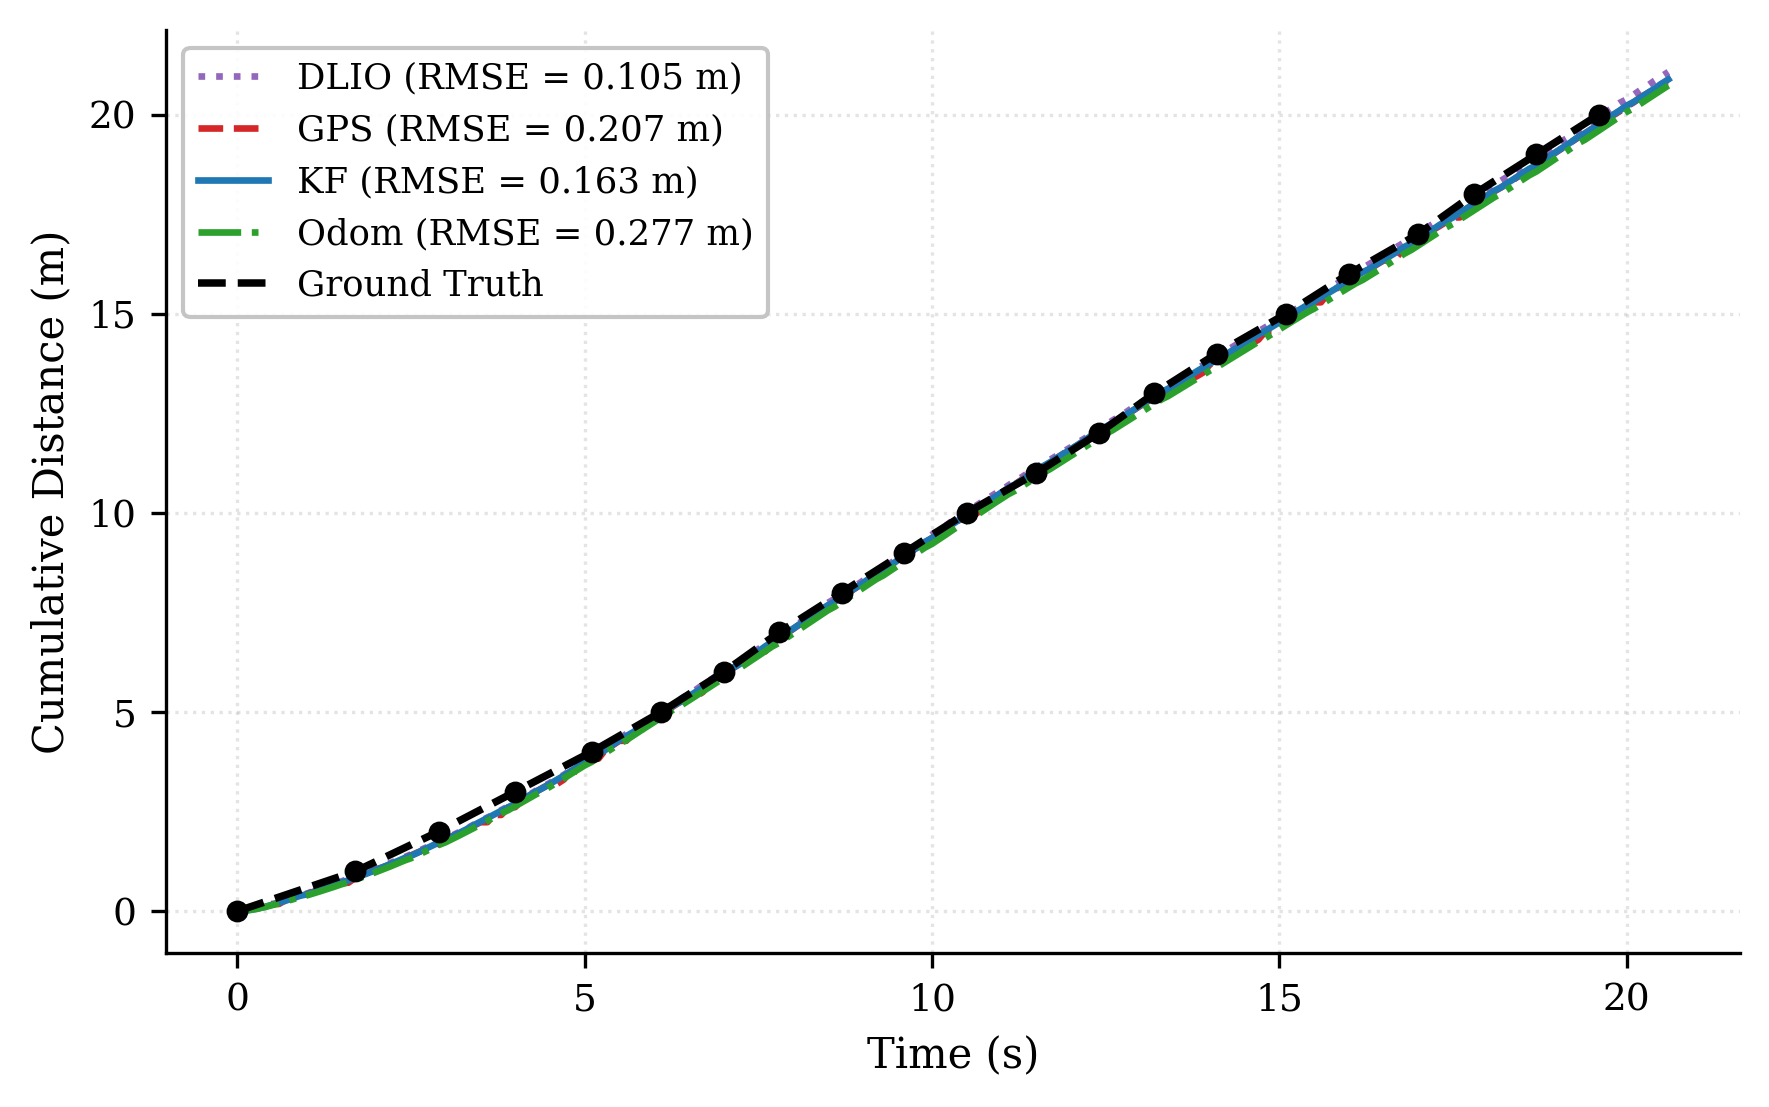
\includegraphics[width=\textwidth]{gambar/kalman_log_7_cumulative_distance.png}
        \caption{Data aktual posisi terhadap waktu}
        \label{fig:gt_dist}
    \end{subfigure}
    \hfill
    \begin{subfigure}[b]{0.48\textwidth}
        \centering
        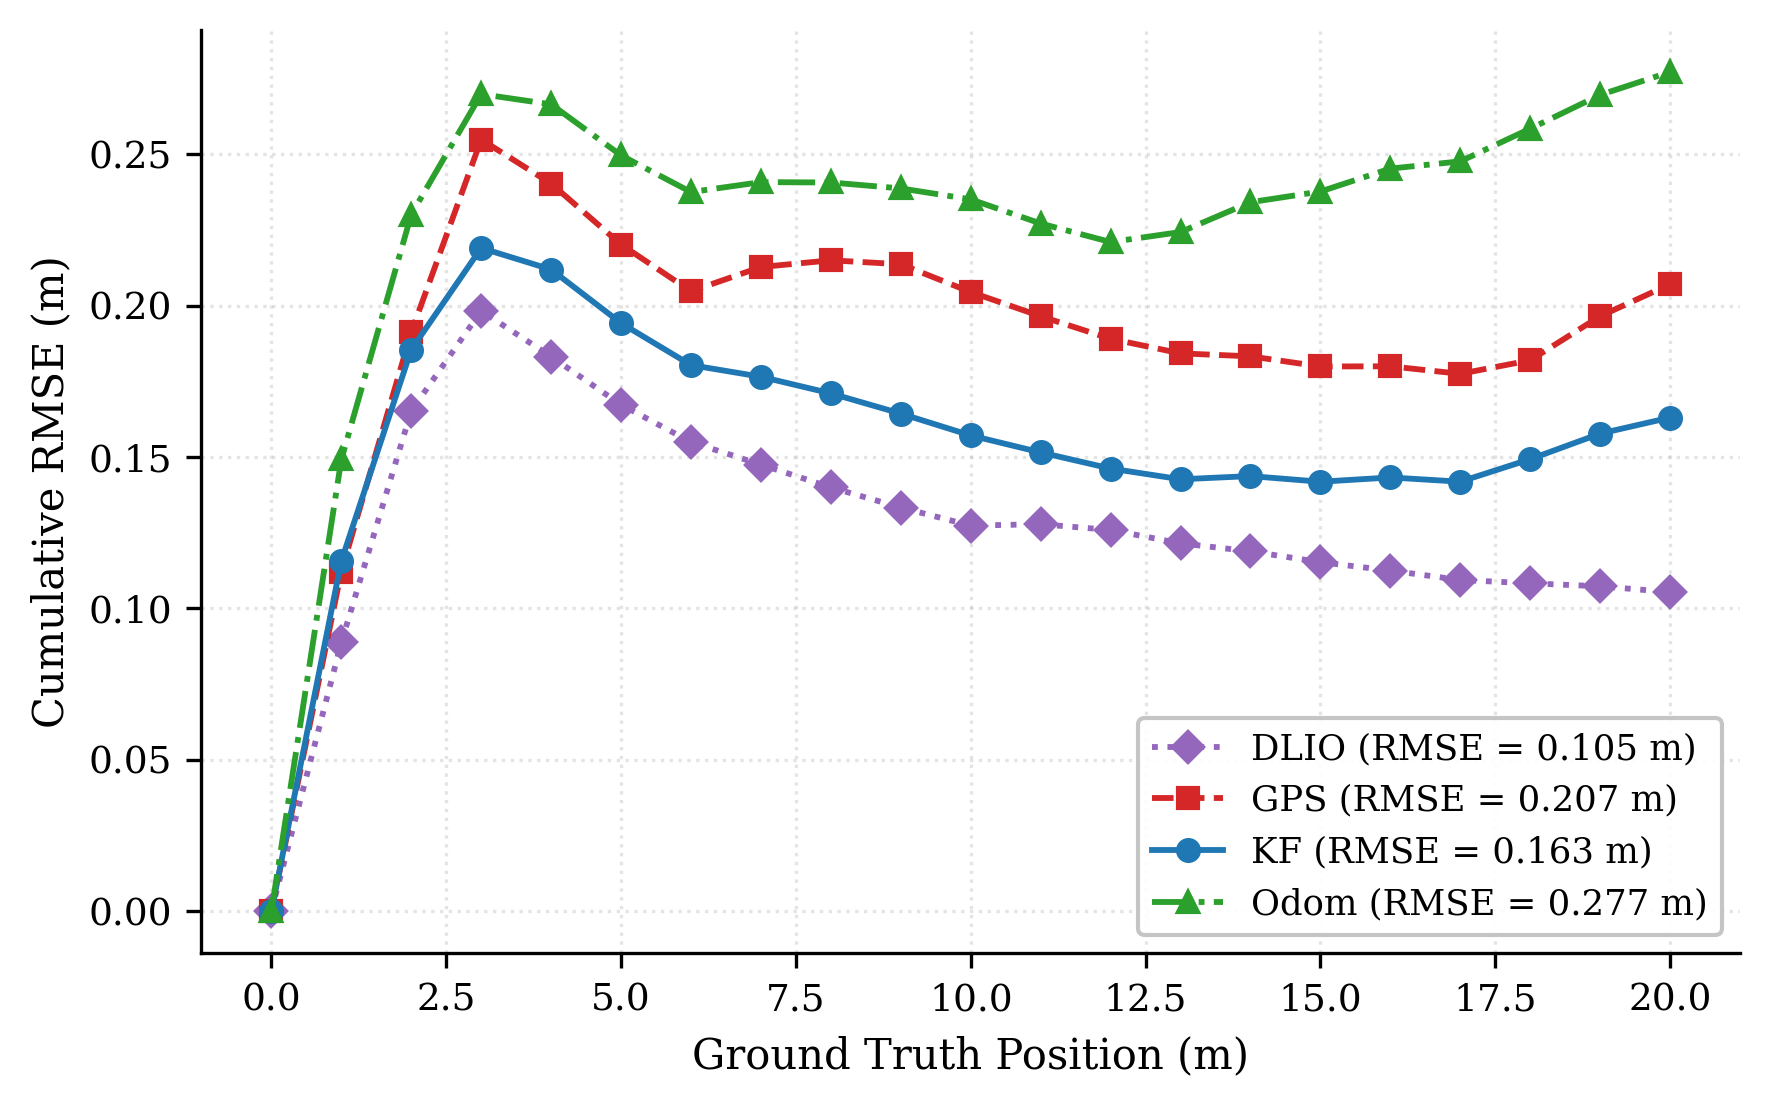
\includegraphics[width=\textwidth]{gambar/kalman_log_7_cumulative_rmse.png}
        \caption{RMSE terhadap data aktual posisi}
        \label{fig:gt_rmse}
    \end{subfigure}
    
    \medskip
    
    \begin{subfigure}[b]{0.6\textwidth}
        \centering
        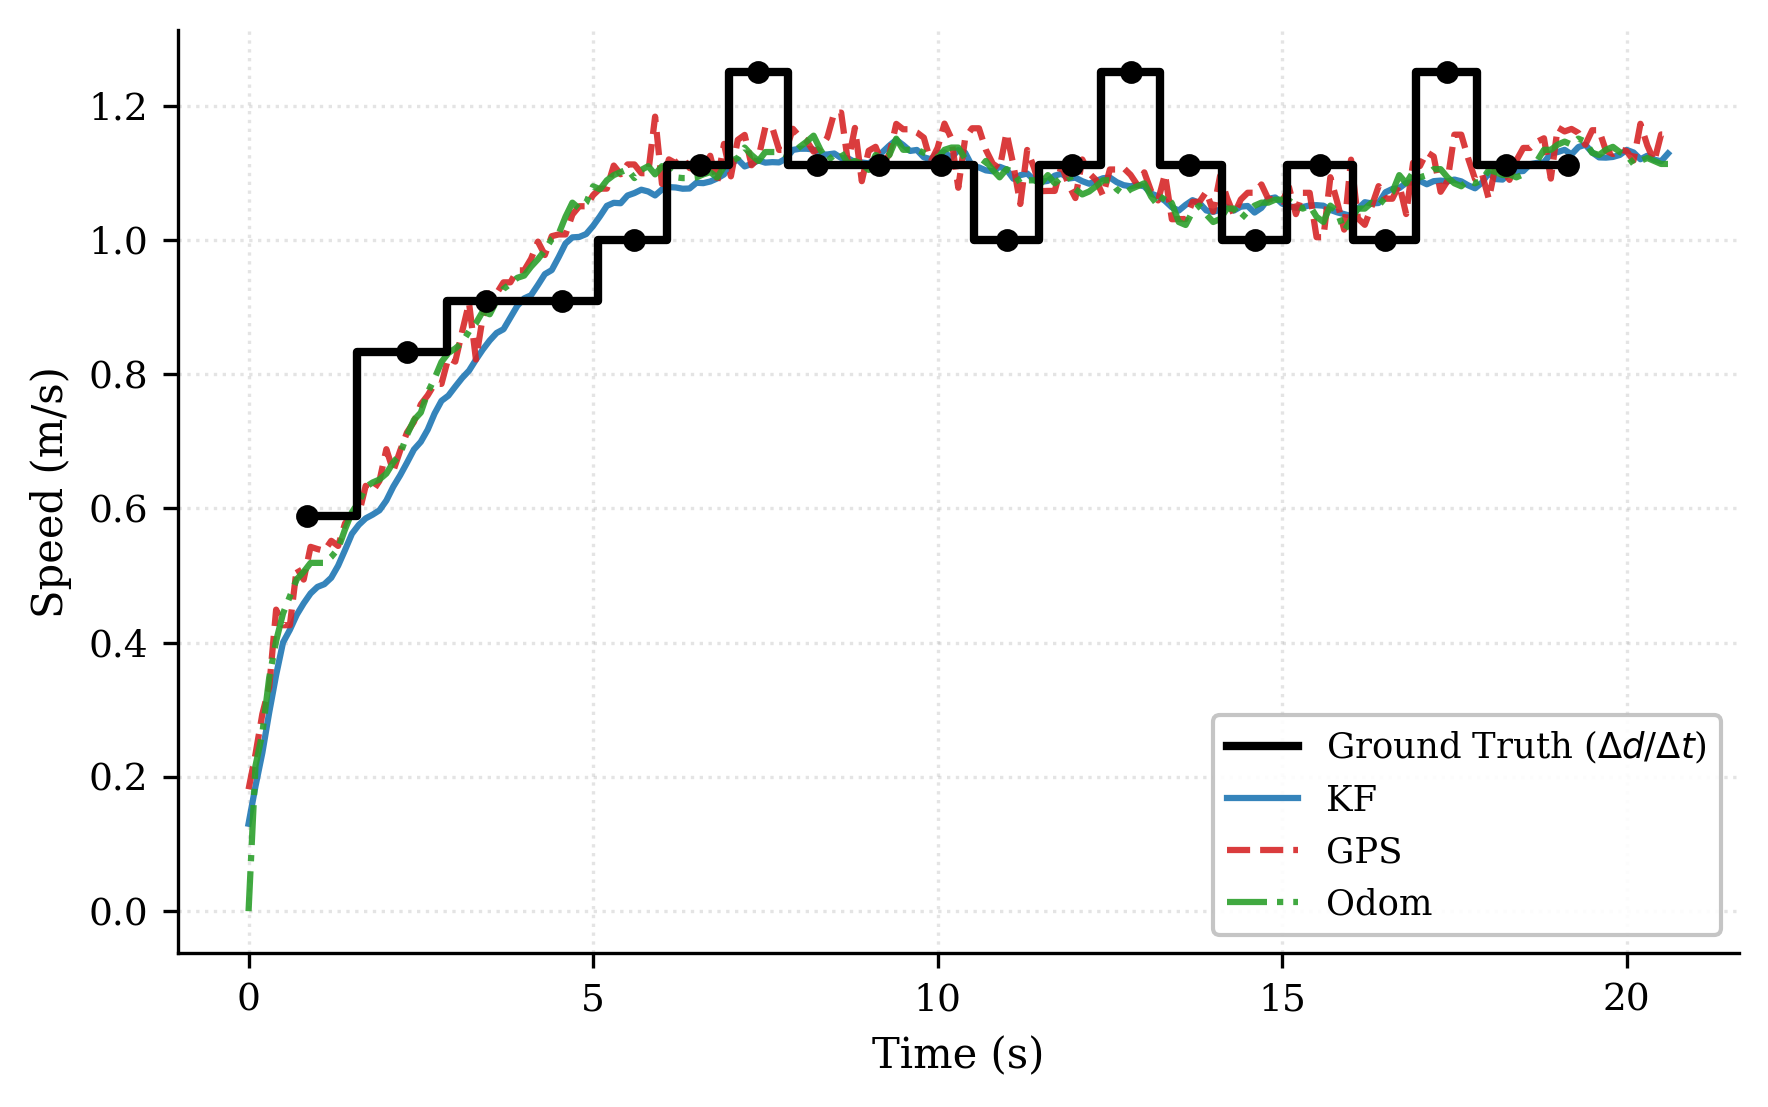
\includegraphics[width=\textwidth]{gambar/kalman_log_7_velocity.png}
        \caption{Kecepatan terhadap waktu}
        \label{fig:gt_vel}
    \end{subfigure}
    \caption{Visualisasi data aktual pada iterasi 2 (0--20 m, 19,6 s).}
    \label{fig:gt_analysis}
\end{figure}

\subsubsection{Pengujian Performa Kalman Filter terhadap Metode Pembanding DLIO}
\label{sec:pengujian_kf_dlio}

Berdasarkan hasil pengujian sebelumnya, DLIO memiliki akurasi posisi yang paling tinggi dengan RMSE rata-rata 0,134 m terhadap data aktual.
Oleh karena itu, DLIO dipilih sebagai \emph{base line} untuk evaluasi lebih lanjut terhadap KF pada rute panjang dan kompleks.
Pengujian dilakukan sebanyak 6 iterasi dengan berbagai kondisi jalan lurus, belokan, dan area dengan degradasi GPS kemudian diukur RMSE estimasi posisi Kalman Filter terhadap metode pembanding DLIO yang ditunjukkan pada Tabel \ref{tab:rmse_csv}.

\begin{table}[H]
\centering
\footnotesize
\caption{RMSE posisi terhadap DLIO pada 6 rute dengan panjang yang berbeda}
\label{tab:rmse_csv}
\begin{tabular}{l c c c c}
\hline
\textbf{Rute} & \textbf{Jarak DLIO (m)} & \textbf{RMSE KF (m)} & \textbf{RMSE GPS (m)} & \textbf{RMSE Odom (m)} \\
\hline
robotika                     & 479,8   & 0,4366 & 0,4707 & 1,0016 \\
k1mart - tower 1             & 611,0   & 0,8546 & 0,9432 & 0,9251 \\
robotika - research center 1 & 736,2   & 0,5063 & 0,7305 & 2,2122 \\
tower1 - manarul ilmi        & 1528,5  & 0,6554 & 1,0398 & 1,6158 \\
robotika - research center 2 & 1311,0  & 0,5218 & 0,6587 & 1,4325 \\
robotika - k1mart            & 3431,6  & 0,8759 & 0,9644 & 8,5883 \\
\hline
\end{tabular}
\end{table}

Hasil menunjukkan bahwa Kalman Filter memiliki RMSE yang lebih rendah daripada GPS dan odometri pada semua rute jalan.
Odometri menunjukkan performa yang bervariasi, dengan RMSE sangat tinggi pada segmen robotika - k1mart sebesar 8,59 m.

Untuk menguji ketahanan sistem terhadap degradasi GPS, dilakukan dengan melewati area jalan rektorat, tepat di depan lobi utama yang dinaungi oleh struktur kanopi beton yang menyebabkan degradasi sinyal GPS secara signifikan.
Pengujian dilakukan sebanyak 9 iterasi dengan variasi waktu henti kendaraan. Tabel~\ref{tab:rektorat} menyajikan hasil pada setiap iterasi.

\begin{table}[H]
\centering
\footnotesize
\caption{Performa KF pada 9 iterasi area Rektorat dengan variasi waktu henti}
\label{tab:rektorat}
\begin{tabular}{l c c c c c c}
\hline
\textbf{Loop} & \textbf{Durasi (s)} & \textbf{Waktu Henti (s)} & \textbf{RMSE KF (m)} & \textbf{RMSE GPS (m)} & \textbf{RMSE Odom (m)}\\
\hline
1  & 82,4  & 0     & 1,5160 & 3,2440 & 1,1003 \\
2  & 128,2 & 0     & 1,0723 & 2,4860 & 0,8895 \\
3  & 133,5 & 3,3   & 1,5636 & 2,7912 & 2,6562 \\
4  & 132,7 & 5,5   & 1,3102 & 2,5291 & 2,2908 \\
5  & 136,9 & 7,0   & 1,2303 & 3,6435 & 1,7799 \\
6  & 136,0 & 9,5   & 1,1845 & 3,0228 & 1,4159 \\
7  & 152,9 & 12,1  & 1,3440 & 4,0658 & 1,1335 \\
8  & 164,2 & 20,4  & 1,1081 & 6,8257 & 0,8911 \\
9 & 174,9 & 20,8  & 1,1960 & 9,4282 & 0,8915 \\
\hline
\end{tabular}
\end{table}

Pada seluruh iterasi, Kalman Filter menunjukkan ketahanan yang cukup baik terhadap degradasi sinyal GPS dengan rentang RMSE 1.07--1,56 m, yang jauh lebih baik dibandingkan dengan GPS yang mengalami peningkatan RMSE hingga 9,43 m.

Gambar~\ref{fig:kf_dlio_comparison} menampilkan perbandingan lintasan KF terhadap DLIO pada kondisi normal (segmen \texttt{robotika}) dan kondisi degradasi GPS (area Rektorat).

\begin{figure}[H]
    \centering
    \begin{subfigure}[b]{0.48\textwidth}
        \centering
        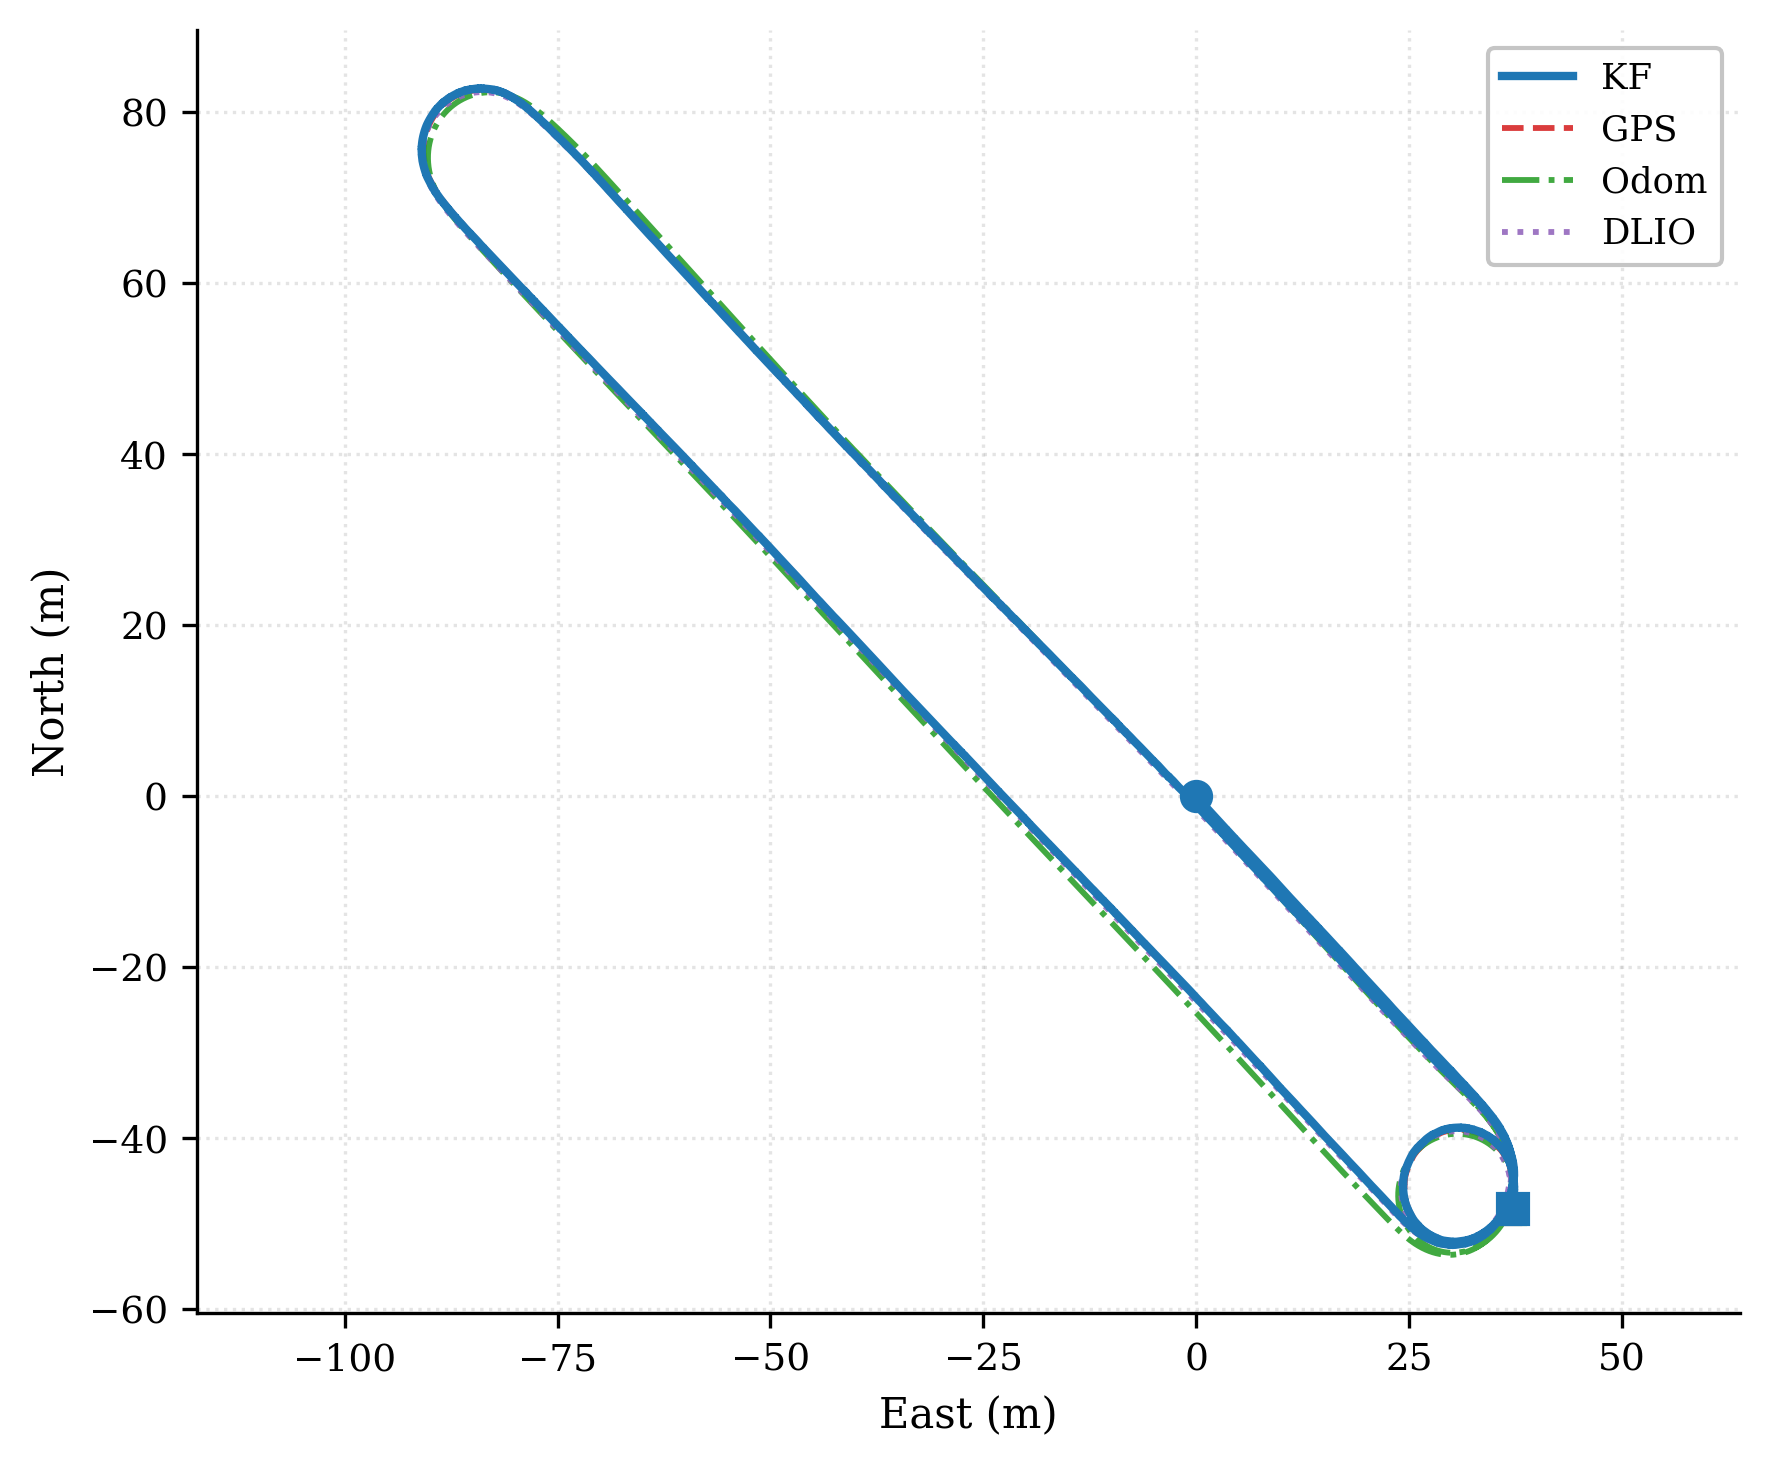
\includegraphics[width=\textwidth]{gambar/robotika_trajectory.png}
        \caption{Area robotika (GPS normal)}
        \label{fig:kf_normal}
    \end{subfigure}
    \hfill
    \begin{subfigure}[b]{0.48\textwidth}
        \centering
        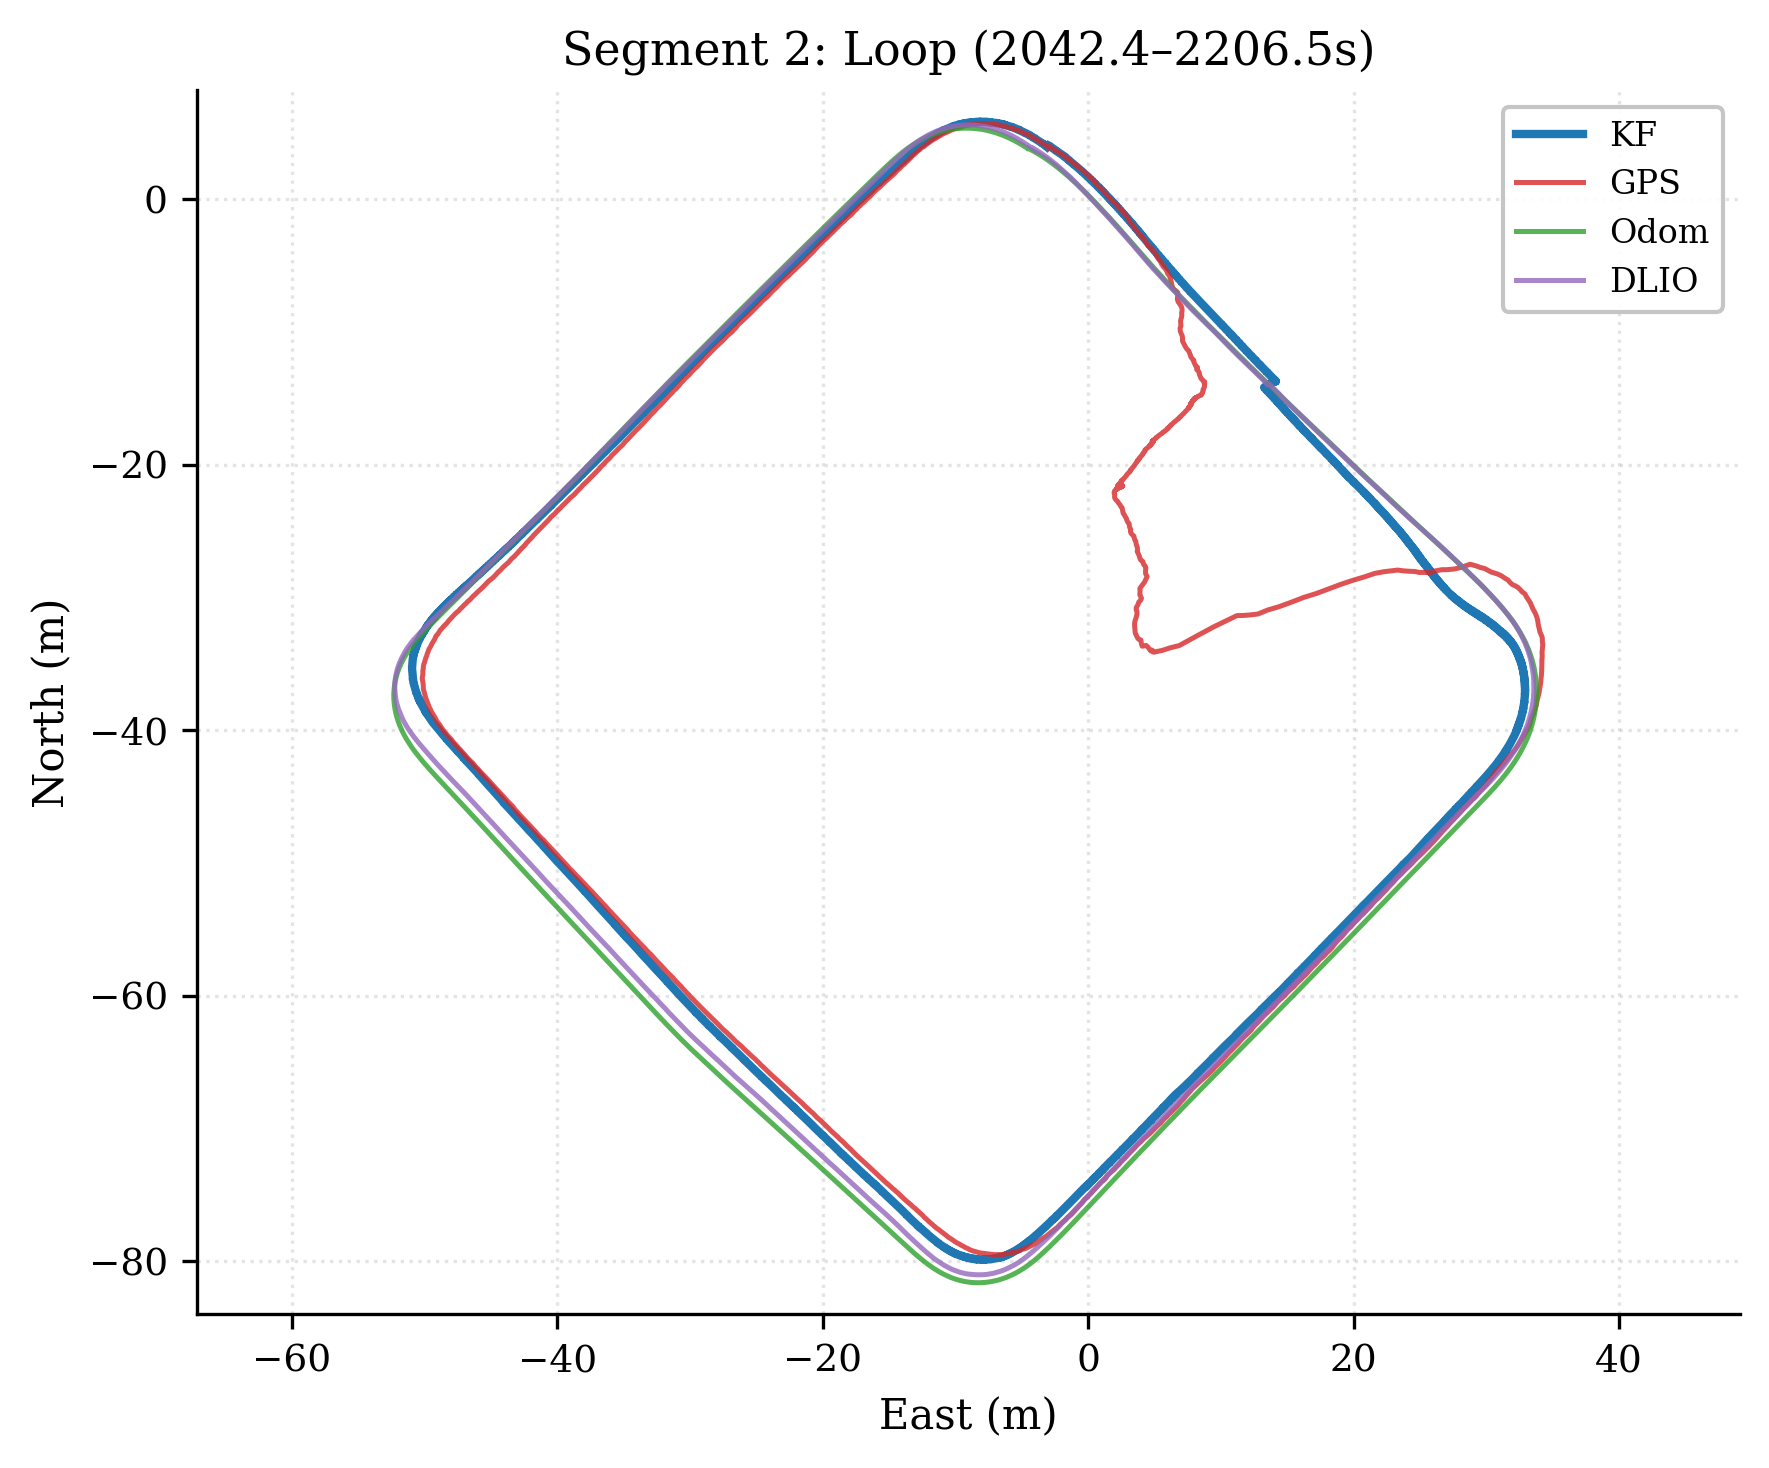
\includegraphics[width=\textwidth]{gambar/rektorat_seg_02_loop.png}
        \caption{Area Rektorat (GPS degradasi)}
        \label{fig:kf_rektorat}
    \end{subfigure}
    \caption{Perbandingan performa KF terhadap DLIO pada kondisi normal dan degradasi GPS.}
    \label{fig:kf_dlio_comparison}
\end{figure}

\subsubsection{Karakterisasi Akurasi Arah Kendaraan (Sudut Hadap)}
\label{sec:akurasi_heading}

Akurasi arah kendaraan atau sudut hadap dievaluasi dengan membandingkan data orientasi yaw dari IMU terhadap arah kendaraan yang diukur oleh GPS dengan referensi utara sejati Bumi (kutub utara geografis).
Pengujian dilakukan pada sirkuit ITS dengan kondisi terbuka tanpa halangan pohon untuk memastikan kualitas sinyal GPS yang optimal.
Data sudut hadap dan akurasinya didapatkan dari data GPS dengan format NMEA yang disajikan dalam log CSV sebanyak 19.894 sampel dengan durasi perekaman sekitar 330 detik.
Tabel~\ref{tab:head_acc_dist} menunjukkan distribusi akurasi sudut hadap dari seluruh sampel.

\begin{table}[H]
\centering
\footnotesize
\caption{Distribusi akurasi sudut hadap pada sirkuit terbuka}
\label{tab:head_acc_dist}
\begin{tabular}{l c c c}
\hline
\textbf{Rentang (derajat)} & \textbf{Jumlah} & \textbf{Persentase}\\
\hline
0,0 -- 0,5   & 28    & 0,14\%  \\
0,5 -- 1,0   & 2245  & 11,28\% \\
1,0 -- 2,0   & 9297  & 46,73\% \\
2,0 -- 5,0   & 7048  & 35,43\% \\
5,0 -- 10,0  & 343   & 1,72\%  \\
$>$ 10,0     & 933   & 4,69\%  \\
\hline
\end{tabular}
\end{table}

Sebanyak 58,2\% sampel memiliki akurasi sudut hadap di bawah 2\textdegree\ dan 93,6\% di bawah 5\textdegree.
Untuk evaluasi akurasi orientasi yaw IMU, dilakukan RMSE terhadap sudut hadap GPS dengan beberapa kondisi batasan untuk menyaring sampel yang valid.
Tabel~\ref{tab:heading_rmse} menyajikan hasil perhitungan RMSE dengan variasi kondisi batasan.


\begin{table}[H]
\centering
\footnotesize
\caption{RMSE orientasi yaw IMU terhadap sudut hadap GPS dengan variasi batasan sampel}
\label{tab:heading_rmse}
\begin{tabular}{l c c}
\hline
\textbf{Kondisi Batasan} & \textbf{Sampel} & \textbf{RMSE (deg)} \\
\hline
Semua sampel                                & 19.894 & 13,27 \\
kecepatan $>$ 0,5 m/s                    & 19.191 & 5,31 \\
kecepatan $>$ 1,0 m/s                    & 19.100 & 2,22 \\
kecepatan $>$ 1,0 \& akurasi sudut hadap $<$ 5\textdegree  & 18.618 & 1,70 \\
kecepatan $>$ 1,0 \& akurasi sudut hadap $<$ 2\textdegree  & 11.570 & 1,13 \\
kecepatan $>$ 1,0 \& akurasi sudut hadap $<$ 1\textdegree  & 2.273  & 0,67 \\
\hline
\end{tabular}
\end{table}

Tanpa menggunakan batasan, RMSE orientasi yaw IMU terhadap sudut hadap GPS sangat tinggi sebesar 13,27\textdegree\.
Kemudian dengan batasan kecepatan $>$ 1,0 m/s dan akurasi sudut hadap $<$ 1\textdegree, RMSE turun drastis menjadi 0,67\textdegree\ pada 2.273 sampel.
Gambar~\ref{fig:heading_plots} menampilkan visualisasi data sudut hadap berupa histogram akurasi sudut hadap dan persebaran orientasi yaw IMU terhadap sudut hadap GPS.

\begin{figure}[H]
    \centering
    \begin{subfigure}[b]{0.48\textwidth}
        \centering
        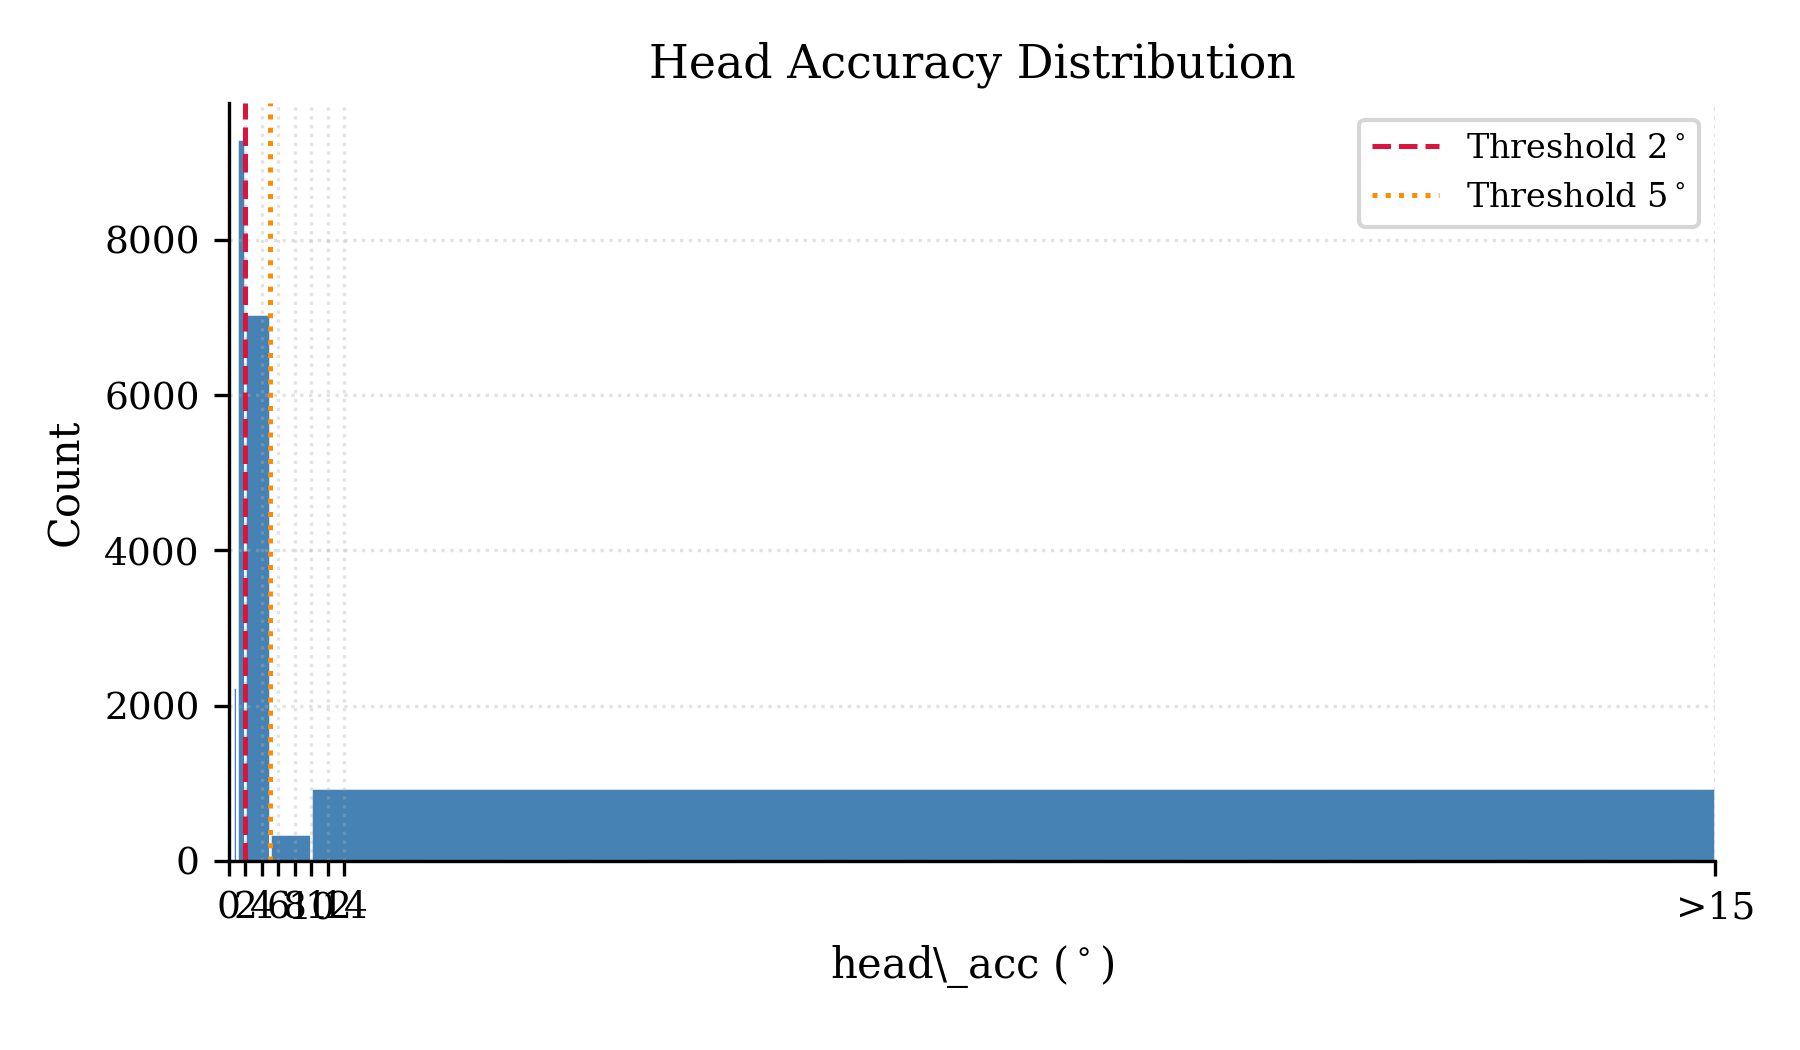
\includegraphics[width=\textwidth]{gambar/kalman_log_13_hist_head_acc.png}
        \caption{Histogram akurasi sudut hadap GPS}
        \label{fig:hist_head_acc}
    \end{subfigure}
    \hfill
    \begin{subfigure}[b]{0.48\textwidth}
        \centering
        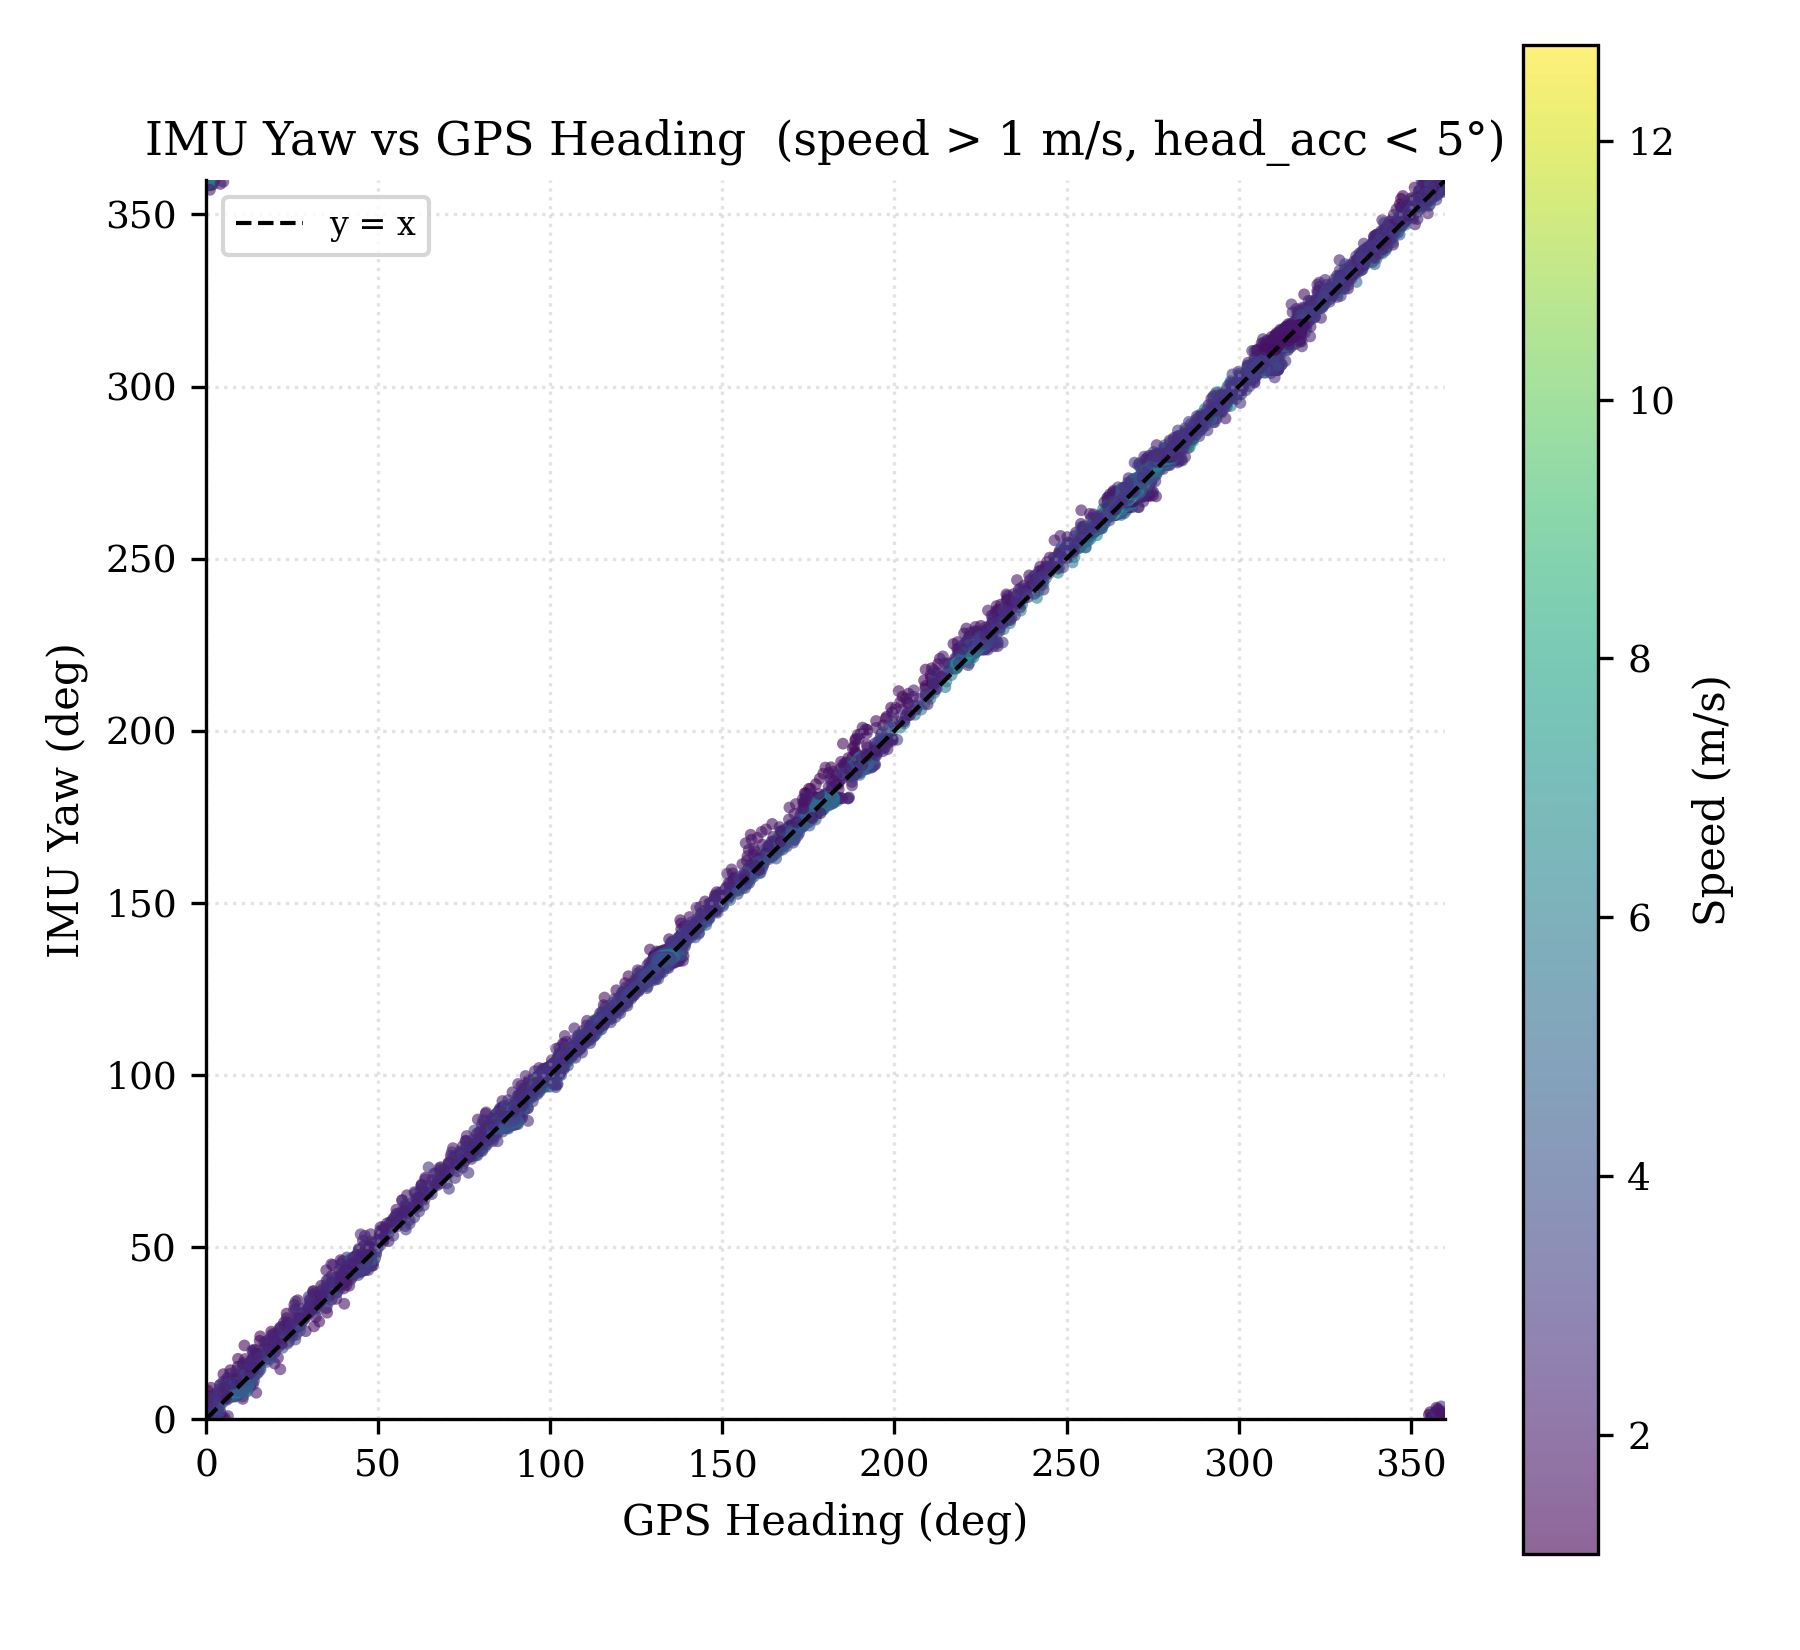
\includegraphics[width=\textwidth]{gambar/kalman_log_13_scatter_yaw.png}
        \caption{Yaw IMU terhadap sudut hadap GPS}
        \label{fig:scatter_yaw}
    \end{subfigure}
    \caption{Distribusi akurasi sudut hadap dan korelasi yaw IMU terhadap sudut hadap GPS pada sirkuit terbuka.}
    \label{fig:heading_plots}
\end{figure}